\chapter{Access Control Analysis}
\chaptermark{Access Control Analysis}
\label{ch:accesscontrol}

\section{Introduction}
Smart contracts deployed on permissionless blockchains, such as Ethereum, are accessible to any
user in a trust-less environment.
Therefore, most smart contract applications implement access control policies to protect their
valuable assets from unauthorized accesses.
The correctness of such policies is critical for maintaining smart contract security.
For example, suicidal contracts~\cite{nikolic2018finding} is a class of vulnerable smart contracts
without proper access control to the ``\texttt{selfdestruct}'' operations, which appear in around
20\% of unique smart contracts~\cite{oyente}.
Another high-profile victim due to vulnerable access control policy is the Parity Wallet.
The wallet was hacked through two different attack vectors resulting in the stolen of \$30M USD and
the frozen of \$100M USD, respectively.
The Parity Wallet consumes a library contract, called WalletLibrary, to implement the basic
functionality of a wallet.
Anybody can deposit money into the wallet, but only the contract owner can withdraw the funds.
The first attack vector exploited the unprotected initialization function to set the attacker as
the contract owner and finally withdrew a large sum of money deposited by other wallet users.
The root cause of this attack is that an unauthorized user can bypass the contract rule rather than
the intended user access.

A difficulty in validating the conformance to such policies, i.e., whether the contract
implementation adheres to the expected behaviors, is the lack of policy specifications. The
current practice is to implement intended access control policies with ad-hoc
Solidity~\cite{solidity} (i.e., the programming languages used to develop Ethereum smart contracts)
idioms, such as the ``\texttt{require}''statements, to check if the address of a user is in a
predefined whitelist.
Many security vulnerabilities mentioned earlier are results from this ad-hoc approach.
In particular, when the number of roles and the complexity of access patterns increase, it becomes
fairly easy for contract developers to make mistakes and introduce bugs causing security
vulnerabilities.

\begin{figure}[t]
	\centering
	\includegraphics[width=\linewidth]{Figures/Chapter4/SPconIllustration-crop.pdf}
	\caption{Illustration of the time-travel-based security policy validation.}
	\label{fig:time-travel}
\end{figure}

In this chapter, we would like to address this problem by relying on past transactions of a contract
to recover a \emph{likely} access control model, which can then be validated against various
security rules and identify potential bugs related to user permissions.
We plan to implement a security policy validator powered by ``time traveling'' through transaction
histories.
As is shown in \cref{fig:time-travel}, the key idea is that, because of the transparency and
immutability of blockchain transactions, the transaction histories of a smart contract application
from its initial deployment up to today are always available on the blockchain.
The historical transactions of a smart contract contain benign user behaviors, assuming the
contract is not yet attacked by any malicious party.
Due to the unique nature of DApps, we can safely assume that the history of a smart contract is
\emph{clean}, if it is still \emph{alive}, i.e., not being destructed or abandoned.
Therefore, we are able to reverse engineer an access control model which is permissible enough to
subsume all historical transactions.
Since historical transactions only under-approximate the behaviors allowed by the contract
implementation, by validating the recovered model against the actual contract implementation, we
will be able to discover discrepancies, indicating potential future violations of security policies.

\begin{figure}[!t]
	\centering
	\scalebox{0.6}{
		%\begin{multicols}{2}
\begin{lstlisting}[language=Solidity]
	pragma solidity ^0.5.0;
	
	contract Dicether{
		
		address owner, server;
		bool activated = false,  paused = true;	
		enum Game{ENDED, ACTIVE, USECANCEL, SERVERCANCEL};
		mapping(address=>Game) games;
			
		constructor(address _serverAddress) public
		{		
				owner = msg.sender;	
				server = _serverAddress;
		}
		// Pause contract 
		function pause() public onlyOwner onlyNotPaused
		{
				paused = true;
		}    
		// Unpause contract 
		function unpause() public onlyOwner onlyPaused onlyActivated
		{
				paused = false;
		}
		function activate() public onlyOwner onlyNotActivated
		{
				activated = true;
		}
		function transferOwnership(address _newOwner) public onlyOwner 
		{
				owner = _newOwner;	
		}
		function transferProfitToHouse() public{
			// transfer profit
		}
	
		// Create game 
		function createGame() public onlyNotPaused payable
		{
				require(games[msg.sender]==ENDED);
				games[msg.sender] = ACTIVE;
		}
		// Cancel game
		function userCancelGame() public payable
		{
				require(games[msg.sender]!=ENDED);
				if (games[msg.sender]==ACTIVE){
						games[msg.sender] = USECANCEL;
				}else if (games[msg.sender]==SERVERCANCEL){
						games[msg.sender] = ENDED;
				}else{
						revert();
				}
		}
		// Cancel game
		function serverCancelGame(address _userAddress)	public onlyServer
		{
				require(games[_userAddress]!=ENDED);
				if (games[_userAddress]==ACTIVE){
					games[_userAddress] = SERVERCANCEL;
				}else if (games[_userAddress]==USECANCEL){
					games[_userAddress] = ENDED;
				}else{	revert();	}
		}
		// End game
		function serverEndGame(address userAddress) public onlyServer
		{
				require(games[_userAddress]==ACTIVE);
				games[_userAddress] = ENDED;
		}
		
	}
\end{lstlisting}
%\end{multicols}

	}
	\caption{The abstracted Solidity contract of Dicether.}
	\label{fig:Dicether}
\end{figure}

\section{Motivating Example}
\label{sec:motivationExample}

Dicether is an contract based casino decentralized application running on Ethereum.
It uses a smart contract based state channel implementation to try to provide a fast, secure and fair gambling experience~\cite{Dicether2018}.
Figure \ref{fig:Dicether} shows the abstracted version of \textit{Dicether}.
The constructor function (Line 10) sets the creator, namely \textit{msg.sender} as the contract owner, which is responsible to pause/unpause contract in case of emergency and specifies the server ${server}$ who administrates all games.

In most cases, game players invoke \textit{createGame} to create a gambling game (Line 37) with ether deposition as the game stake,
and once a game approach the deadline, the server will end the game via \textit{serverEndGame} (Line 65) and also distribute the profit to the game player.
Alternatively, the players can cancel their games via \textit{userCancelGame} (Line 43).
If the server also confirm the cancellation via \textit{serverCancelGame}, the game will be ended.
Once the previous game has been ended, the players can create new games and follow the aforementioned procedure as well.

The access control of \textit{Dicether} is complicated.
On the one hand, there are server types of users to perform different tasks such as the \textit{owner}, \textit{server},  \textit{players}.
On the other hand, tasks performed by users should follow a predefined temporal logic, e.g., a player must first create a game, then he/she can cancel the game.
Besides, there exists a lot of uncertainty about the composition of users involved in a running Dicether contract.
First, the exact \textit{owner} and \textit{server} is unknown before contract deployment.
Second, the intended user behavior is unknown even there is  specification about smart contracts and the intended user behavior is usually understood only after large-scale use.

The running \textit{Dicether} contract has more than 9,427 transactions sent by around 400 different users (an Ethereum account can be a user) as of May 2021.
Since \textit{Dicether} is still active, we incline to believe the contract runs as expected by developers and users.
Further, the set of user behaviors in its history provides sufficient knowledge to recover its access control model, i.e., user permission model where includes all intended user behavior.

\section{User Permission Model}
\label{sec:preliminary}
In this section, we will present user permission analysis framework.
We base our user permission model on role-based access control (RBAC) which is a general framework for implementing various security policy.
We focus on three types of information-flow security policy.
(1) Integrity.
The users of low security-level role cannot write to information managed by the users of high security-level role.
(2) Separation of duty. 
There is no information flow between two or more user roles.
(3) Cardinality. 
There is a constraint on the range of roles who can participant in a session.
%\begin{figure}[t]
%	\centering
%	\small
%	\begin{grammar}
%		<Contract> ::= <stateVar>*; <function>*
%
%		<function> ::= <access>*; <statement>*
%
%		<access>   ::= \textbf{require} \text{user has permission}
%		%<userexp> ::= msg.sender | \textbf{hash}(<userexp> [+-] <exp> ) [+-] <exp>
%		%\alt \textbf{read}(<userexp>)
%		%
%		%<exp>	   ::= $\mathbb{C}$ | $\mathbb{N}$ | msg.sender | <state>[+-]<exp> | <exp>[+-]<exp>
%		%\alt \textbf{hash}(<exp>)
%
%		<statement> ::= \textbf{update} \text{contract \textit{stateVar}}
%	\end{grammar}
%
%
%	\caption{Abstraction of access control in smart contracts.}		\label{fig:abstraction}
%\end{figure}
%\subsection{Smart Contract Access Control}
%\label{subsec: accesscontrol}
%Figure~\ref{fig:abstraction} shows a grammar that describes our abstraction
%over access control in a smart contract. A contract consists of state variables
%and functions that access and update these variables.
%At runtime, smart contract access control will check user permission when a user tries to execute a function.
%The state of a smart contract is updated only if a user has permission to do so.
%Because there is no built-in mechanism to implement access control, each smart
%contract implements its own scheme to enforce user permissions,
%creating a need for a verification tool.
%\todo[inline]{Does the sentence above convey your message?}
%\st{However, not every smart contract has implemented proper access control.}
%\st{Therefore, it is necessary to analyze smart contract access control for which we should
%understand the characteristics of users involved in smart contracts.}
%\todo[inline]{CA: What exactly do you mean with the last sentence?}
%\todo[inline]{Liu Ye: Just delete it.}
%%
%Blockchain is often called a distributed ledger recording transactions, consisting of blocks linked by cryptographic hashes and managed by a peer-to-peer network.
%Blockchain can support not only transactions among users but also transactions between users and smart contracts.
%Figure~\ref{fig:smartcontractTransaction} briefly shows smart contract transaction on Ethereum.
%A user (or client) sends transaction to a miner for executing specific contract function after block $n$.
%The miner then reads blockchain state database and run on it the called function whose operation codes are interpreted by Ethereum virtual machine (EVM).
%Later, the blockchain state database transitions and the miner will commit the new state database to a mined block that will append as block $n+1$ after validation.
%Finally, the user get receipt to confirm transaction result including its status, event logs, ether transferred as well as gas\footnote[3]{Gas is the fee paid to the miner by transaction sender.} consumption.
%If the transaction status indicates success, the state of contract will transition to new one. Otherwise, the contract state will remain unchanged.
%\begin{definition}
%	\textbf{Contract State and Transaction.}
%A contract state $\delta$ can be defined by $<Bal, G\_vars>$ where $Bal\in \N$ is the cryptocurrency balance owned by contract and $G\_vars$ is the values of all the storage variables managed by contract.
%For simplicity, we define a transaction to smart contract as $t\leftarrow <sender, value, func,
%status>$, where $sender$ is an external account to invoke contract's function $func$ and $value$
%is
%the amount of attached ethers correspondingly.
%If the function invocation succeeds, $status$ is ``1''; otherwise, $status$ is ``0''.
%Hereby, the transition types of contract state can be formalized as (a) and (b).
%\begin{align*}
%	(a)\quad\delta \xrightarrow[t.status=0]{t} \delta \quad \quad
%	(b)\quad\delta \xrightarrow[t.status=1]{t} \delta^{'}
%\end{align*}
%In this paper, we focus the transitions of $(b)$ because the state of smart contract does change.
%\end{definition}
%
%%\liu{
%Decentralized applications (DApps) have been rapidly developed and widely adopted in many areas including finance, gambling, exchanges, governance, property and etc..
%The core of DApps are supported using smart contracts for achieving different purpose.
%%How to make a claim that smart contracts are task based.
%For instance, Ethereum Name Service (ENS) use auction contract to provide the service for users bidding different domains;
%Dicether uses contract to maintain houses for users' participation in different gambling games;
%and CryptoKitties uses contract to organize blockchain stores for the purchase, breeding and
%selling or siring of unique digital pets implemented as non-fungible tokens (NFTs).
%Most likely DApps are designed around items like games, domains, pets and etc., and DApp users also mainly take actions to these items for benefits.
%Therefore, it is practical to learn the DApps design through the observation of user actions.
%%}

%
%On the other hand, the purpose of the transactions subjects to the invoked functions.
%Most smart contracts allow for users invoking same functions again and again to achieve their
%business.
%Based on the function invocation patterns, we summarize three basic transition types of smart contract shown in fig.~\ref{fig:contracttypes} which is described in the following.
%\begin{itemize}
%	\item \textbf{Flat.} Flat smart contract shows a single process with no repeated function invocations.
%	\item \textbf{Cycle.} Cycle smart contract shows a repeated pattern of function invocation.
%	A circle of cycle represents a process and cycle means different processes are performed orderly.
%	\item \textbf{Parallel.} Parallel smart contract also shows a repeated pattern and each separated transition chain represents a process.
%	In this case, different processes are performed relatively independently in parallel manner.
%\end{itemize}
%Generally, smart contracts attract the interactions from many users into different processes either via the parallel manner or the cycle manner.
%For example, Dicether of Fig.~\ref{fig:gameChannel} has a parallel transition type, where
%the processes are either \textcircled{1} or \textcircled{2} or \textcircled{3} running independently for different gambling games.
%The former is used for smart contract initialization by user of \textit{role4} through a series of function invocation: \textit{activate} $\rightarrow$ \textit{addHouseStake} $\rightarrow$ \textit{unpause} $\rightarrow$ etc..
%Meanwhile, the latter is used by users of \textit{role1} and \textit{role5} to manage game session including creation, cancellation and ending operations shown in fig.~\ref{fig:dicether-SessionModel}.

%\input{Figures/Chapter4/typesOfSmartContract}


\subsection{Role-Based Access Control Model}
Role-based Access control (RBAC) has been well studied in the last twenty years since the establishment of the NIST RBAC standard in 1995~\cite{sandhu2000nist}.
We borrow the standard RBAC definition~\cite{sandhu1998} here.
\begin{definition}
	\label{def: RBAC}
	\textbf{RABC.} The general RBAC model $M$ can be defined in a tuple 
	$(U, R, P, S, \mathit{RH}, \mathit{PA}, \mathit{UA})$.
	%   $(U, R, P, \mathit{RH}, \mathit{PA}, \mathit{UA})$.
	$U$, $R$, $P$ and $S$ are users, roles, permissions and sessions respectively.
	$U$, $R$ and $P$ are users, roles and permissions respectively.
	$\mathit{RH} \subseteq R \times R$ is a partial order on $R$ called the role hierarchy, usually
	written as ``$\succ$''.
	$\mathit{PA} \subseteq P \times R $ is the permission-to-role assignment relation while
	$\mathit{UA} \subseteq U \times R$ the user-to-role assignment relation.
	And $U \times S \times 2^{R_\mathit{active}\subseteq\{r|x \in U \land (x,r) \in \mathit{UA}\}}$ is the role activation for each user in a session, where a session is the unit of access control.
\end{definition}


Notice that RBAC is policy neutral and can implement different security policies mainly owing to the generality of permission concept.
%Moreover, even though a session between one or more users is the unit of access control,
Similarly, the context of a session varies a lot between different contracts.
%For simplicity, in this paper, we consider the managed items by DApp smart contracts as the context of session without loss of generality.

%However, the sessions can be represented by the processes from the three transition types of smart contract in Sec.~\ref{subsec: transaction}.
%A session of smart contract is a process.
%}
%A session model is to show how users exercise their permissions in sessions.
%Because different users play different roles in each session,
%the session model can demonstrate the interplay patterns between users around a concrete item.
%We use this session model to extract some security policies which is discussed in Sect.~\ref{subsec: policy}.
%Further, based on a session model, we can infer the RBAC constraints which is detailed in Sect.~\ref{subsec: constraints}.


%\subsection{Session-Based State Machine Model}
\begin{definition}
	\textbf{Session}.
	A session is actually the unit of multi-party communication between users and contract.
	A session is usually implemented as a stateful resource of smart contract where each session is assigned a unique identifier, i.e., \textit{id}. 
	Meanwhile, a session transits to a state by user activities, i.e., user calling contract functions which take \textit{id} as either input or output.
\end{definition}
\begin{definition}
	\textbf{Role-Based Session Finite State Machine.} 
	A session usually has a limited number of states which can be interpreted by a finite state machine.
	A role-based session finite state machine, \textit{SFSM}, can be defined as a 5-tuple $(S, s_0, F, L,T )$. $S$ is a set of finite states of sessions, $s_o \in S$	is the initial state, and $F \subseteq S$ is the set of final states. $L$ is the set of user activities, $(role, action)\in L$ while $T$ is the set of transitions and $T \subseteq S \times L \times S$.
	And \textit{role} is defined in Definition~\ref{def: RBAC} while \textit{action} is the invocation of a concrete contract function. 
\end{definition} 
%
\subsection{Security Policies on Top of User Permissions}
%\subsection{Separation of Duty and Cardinality Constraints}
\label{subsec: policy}
In this section, we present an overview of security policies: (1) integrity, (2) separation of duty, and (3) cardinality in Fig.~\ref{fig: policy}. 
All security policies focus on information flow between roles.
Note that each arrow represents information flow direction and ellipse represents user role.
Information integrity requires information flows from the role of higher security level to the role of low security level.
And separation of duty requires no information flows between two roles.
Cardinality requires no other roles can involve in the information flow inside session.
\begin{figure}
\centering
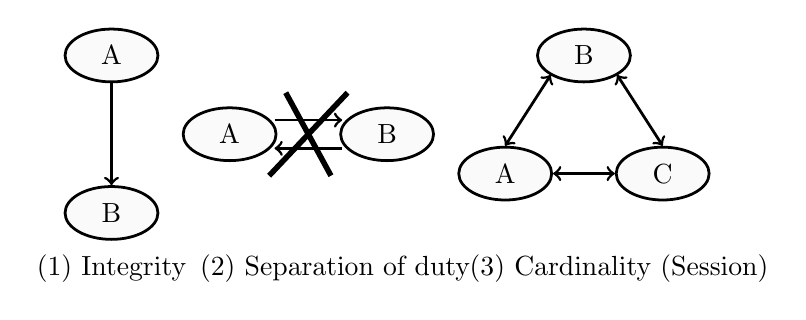
\begin{tikzpicture}[rounded corners=2pt, line width=1pt]
	\tikzstyle{role}=[fill={rgb:black,1;white,50}, ellipse,draw, text width=0.6cm, text centered]
	\draw (0, 2) node[role]  (A1) {A};
%	\draw (0, 2) ellipse (2cm and 1cm) ;
	\draw (0, 0)	node[role] (B1) {B};
	\draw ([yshift=-10pt]B1.south) node[] (integrity) {(1) Integrity};
	
	\draw[->] (A1.south) -- (B1.north);
	\draw (1.5, 1)  node[role] (A2)  {A};
	\draw (3.5, 1)  node[role] (B2) {B};
	
	\draw[->]  ([yshift=-2pt, xshift=4pt]A2.north east) -- ([yshift=-2pt, xshift=-4pt]B2.north west);
	\draw[<-] ([yshift=2pt, xshift=4pt]A2.south east) -- ([yshift=2pt, xshift=-4pt]B2.south west);
	
	\draw [line width=2pt] ([yshift=15pt, xshift=3pt]A2.east) -- ([yshift=-15pt, xshift=-3pt]B2.west);
	\draw [line width=2pt] ([yshift=-15pt, xshift=-3pt]A2.east) -- ([yshift=15pt, xshift=3pt]B2.west);
	
	\draw ([xshift=50pt]integrity.east) node[] (separation) {(2) Separation of duty};
	
	\draw (5.0, 0.5)  node[role] (A3) {A};
	\draw (6, 2)  node[ role] (B3) {B};
	\draw (7, 0.5)  node[ role] (C3) {C};
%	\draw[black, semitransparent] (6, 1) circle[radius=1.8] ;
	\draw[<->]  (A3.east) -- (C3.west); 
	\draw[<->]  (C3.north) -- ([yshift=3pt, xshift=12pt]B3.south);
	\draw[<->]  ([yshift=3pt, xshift=-12pt]B3.south) -- (A3.north);

	\draw ([xshift=50pt]separation.east) node[] {(3) Cardinality (Session)};
	
\end{tikzpicture}
\caption{Overview of security policy.}
\label{fig: policy}
\end{figure}
%\begin{figure}
%	\centering
%\includegraphics[scale=0.45]{Figures/Chapter4/securitypolicy.pdf}
%\caption{Overview of security policy. Each arrow line represents an information flow direction.}
%\label{fig: policy}
%\end{figure}

%To express these information flow policies, there are a lot of approaches ...

For static enforcement of security policy, 
most information-flow properties are linear-time properties.
However, LTL cannot express these properties because LTL can only express trace properties while information-flow properties need the comparison of multiple execution traces~\cite{rabe2016temporal}.
In~\cite{rabe2016temporal} the authors proposed HyperLTL which extends LTL with trace quantifiers in order to relate multiple execution traces.
The grammar of HyperLTL is listed below, where $a \in AP$, $AP$ is a finite set of propositional variable; and $\pi$ ranges over trace variables.
\begin{align*}
	\varphi ::&= \quad true \quad |\quad  a_{\pi} \quad | \quad \neg \varphi \quad | \quad \varphi \lor \varphi \quad | \quad \varphi \land \varphi \quad \\
	& | \quad \bigcirc \varphi \quad  | \quad \varphi U \varphi \quad | \quad \varphi R \varphi \quad | \quad \exists \pi . \varphi \quad | \quad \forall \pi . \varphi 
\end{align*}
Moreover, the usual derived temporal operators \textit{eventually} $\Diamond \varphi \equiv true \; U \; \varphi$ and \textit{globally} $\square \varphi \equiv \neg \Diamond \neg \varphi$.
The following HyperLTL property specifies integrity for a high security-level role \textit{h}:
$
\forall \pi. \forall \pi^{'}.\square (I_{h,\pi} = I_{h,\pi^{'}})\implies \square (O_{h, \pi} = O_{h,\pi^{'}})
$, where $\mathit{I}$ and $\mathit{O}$ are the sets of propositions for public inputs and outputs.
And $ I_{h,\pi} = I_{h,\pi^{'}}$ and $O_{h, \pi} = O_{h,\pi^{'}}$ indicates that the atomic propositions $I_h$ and $O_h$ are equal in the path $\pi$ and $\pi^{'}$ at the current point of time. 
This property implies that if the input $I_h$ of high security-level user is same on any two traces, the output $O_h$ of high security-level user remains unchanged. 

However, this strong integrity property does not apply to the dynamic enforcement of security policy of smart contract
since the user of high security-level role can announce its privilege and promote the user of low security-level role to be of high security-level role.
For example, HyperLTL integrity property fails for Dicether. 
As shown in fig.~\ref{fig: HyperLTLfailure},
assuming that there are three users: \textit{a}, \textit{b} and \textit{c}. Initially \textit{a} is of high security level who calls the constructor function of Dicether which sets he/she as the contract owner. 
Take the value of contract owner as the output of \textit{a},
the proposition on the output is a constraint on the owner value. 
the red path shows an execution trace \textit{R}: ``\textit{a} calling constructor function. $\rightarrow$ \textit{a} transfers ownership to \textit{b}. $\rightarrow$ \textit{c} create a game''. 
At the end of trace \textit{R}, the contract owner is \textit{b}.
And the blue path shows an execution trace \textit{B}: ``\textit{a} calling constructor function. $\rightarrow$ \textit{a} transfers ownership to \textit{b}. $\rightarrow$ \textit{b} transfers ownership to \textit{c}''. 
At the end of trace \textit{B}, the contract owner is \textit{c}.
The two execution traces \textit{R} and \textit{B} have same input of \textit{a} 
but the output, i.e., contract owner of \textit{a} is \textit{b} of \textit{R} and \textit{c} of \textit{B} respectively. 
Apparently, the HyperLTL integrity property is violated but \textit{transferownership} has no security risk for that.
The root cause is that the HyperLTL property is not suitable for describing dynamic security policy of smart contracts. 

\begin{figure}
\centering
\small
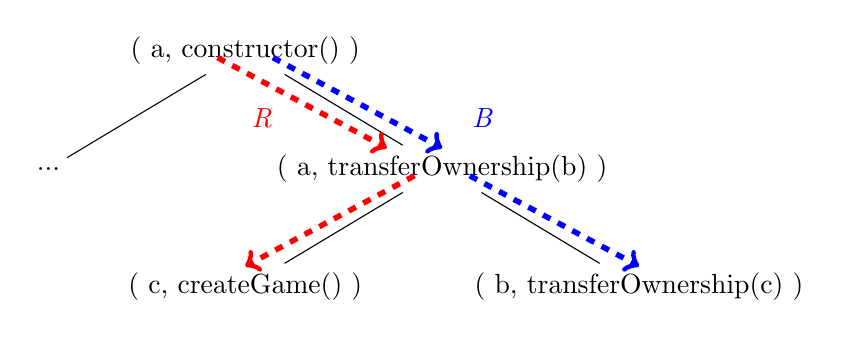
\begin{tikzpicture}
	\node (root) {( a, constructor() )}
	[sibling distance=50mm]
	child {node {...}}
	child {node (transfer1) {( a, transferOwnership(b) )}
		child {node (create) {( c, createGame() )}}
		child {node (transfer2) {( b, transferOwnership(c) )}}
	};
%	\draw [line width=3pt, red] ([yshift=10pt, xshift=-5pt]root.base) -- ([yshift=-10pt, xshift=-5pt]transfer1.base) -- (create.base) ;

	\path [line width=2pt, ->, dashed, blue] ([ xshift=10pt]root.base) edge ([ yshift=10pt]transfer1.base);
	\path [line width=2pt, ->, dashed, blue] ([ xshift=10pt]transfer1.base) edge ([ yshift=10pt]transfer2.base) ;
	
	\path [line width=2pt, ->, dashed, red] ([ xshift=-10pt]root.base) edge ([ yshift=10pt, xshift=-20pt]transfer1.base);
	\path [line width=2pt, ->, dashed, red] ([ xshift=-10pt,]transfer1.base) edge ([ yshift=10pt]create.base) ;
	
	\draw ([xshift=15pt, yshift=10pt]transfer1.north) node[] {\textcolor{blue}{\textit{B}}} ;
	
	\draw ([xshift=-65pt, yshift=10pt]transfer1.north) node[] {\textcolor{red}{\textit{R}}} ;
	
\end{tikzpicture}
\caption{Execution tree of Dicether}
\label{fig: HyperLTLfailure}
\end{figure}

\paragraph{Integrity} 
Therefore, we weakened the HyperLTL property of integrity into a standard LTL property in this work.
The following LTL propery $\varphi_1$ specifies weakened integrity for a high security-level role \textit{h} for smart contract having history $\Gamma$:
\begin{align*}
	\forall \pi^{+}.\square (I_{h,\Gamma} = I_{h,\Gamma \triangleleft \pi^{+}})\implies \square (O_{h, \Gamma} = O_{h, \Gamma \triangleleft \pi^{+}})
\end{align*}

The LTL property can be simplified as $
\square (I_{h}^{0} = I_{h})\implies \square (O_{h}^{0} = O_{h})
$, where $I_{h}^{0}$ and $O_{h}^{0}$ respectively represent the input and the final output of high security-level role on $\Gamma$.
Suppose we have a contract model \textit{M} at the time of $\Gamma$, 
the problem whether $ M \implies \varphi_1$ is of our interest. 


\paragraph{Separation of duty} Similarly, the following LTL property $\varphi_2$ specifies separation of duty given $\pi_{R_s}$ ranging over execution traces by a set of roles $R_s$:
\begin{align*}
	\underset{r\in R_s }{\land} \square (I_{r}^{0} = I_{r})\implies \square (O_{r}^{0} = O_{r})
\end{align*}

%\paragraph{Weakened Separation of duty} The following HyperLTL propery specifies separation of duty given $\pi_{R_s}$ ranging over execution traces by a set of roles $R_s$ for smart contract having history $\Gamma$: \textbf{ Forall} $r\in R_s$,
%\begin{align*}
% \forall \pi^{+}_{R_s}.\square (I_{r,\Gamma} = I_{r, \Gamma \triangleleft \pi^{+}_{R_s}})\implies \square (O_{r, \Gamma} = O_{r,\Gamma \triangleleft \pi^{+}_{R_s}})
%\end{align*}


\paragraph{Cardinality (Session)} The following LTL property $\varphi_3$ specifies cardinality for a set of roles within session $R_c$:
\begin{align*}
	\square (\underset{r\in R_c }{\land} I_{r}^{0} = I_{r})\implies \square ( \underset{r\in R_c }{\land} O_{r}^{0} = O_{r})
\end{align*}


\section{Framework}
\label{sec:framework}
%
\begin{figure*}[t]
	\centering
	\includegraphics[scale=0.45]{Figures/Chapter4/Framework-SPCon.pdf}
	\caption{Workflow of the \spcon Framework.}
	\label{fig:framework}
\end{figure*}
%
%
%\begin{figure*}[t]
%	\centering
%	\includegraphics[scale=0.6]{Figures/Chapter4/ASE21-Framework.pdf}
%	\caption{Workflow of the \spcon Framework.}
%	\label{fig:framework}
%\end{figure*}
In this chapter, we present \spcon, a framework for finding user permission bugs via time travel on transaction history of smart contracts.
\spcon consists of four main stages: (1) RBAC model construction from transaction history,
(2) Security policy inference via information flow analysis of smart contracts,
(3) Testing and (4) Model checking for finding permission bugs and proving security policy respectively.
%Figure~\ref{fig:framework} shows the overall workflow of \spcon.
%The input of \spcon is the transactions history of smart contract 
%while the final output shows the verification result of smart contract access control.
%The \spcon consists of three modules: RBAC model construction, inferring constraints and smart contract verification.
%
%The collected access logs from transactions history are used for two purpose.
%The first purpose is to extract user permission pairs for construction of basic RBAC model.
%The user permission pair is constructed for each successful transaction using the address of external account and the name of called function.
%Role mining process will use these user permission pairs to infer the minimal number of roles and construct the basic RBAC model which has no constraints.
%
%And the second purpose is to infer constraints on the above basic RBAC model.
%Firstly we extract sessions from transactions history based on the transition types of smart contract in Sect.~\ref{subsec: transaction}..
%Each session features a transaction sequence to complete a task.
%For smart contract having many sessions for similar tasks, 
%we believe these sessions are homogeneous so that we can have a session model.
%The model is generated by automata learning accepting sessions and mine roles as input.
%Later, we infer access control constraints in session model such as separation of duty and cardinality constraints on the session model.
%
%Finally, the basic RBAC model and these enabled constraints are used to verify smart contract for vulnerabilities related to access control. 
%The verification is a testing based process and we manually validate the result due to the lack of ground truth.

%\subsection{The Extraction of Smart Contract Access Control Mechanism}

\subsection{The User Role Mining}
\label{subsec: rolemining}
To construct the user model of a smart contract, we need first to identify user roles.
We do this by reverse engineering user roles from the history of the smart contract.
Firstly, we extract user access information where users have successfully called contract functions.
For simplicity, a user access is a 2-tuple $(u, f)$ where $u \in U$ and $f\in \mathit{ABI}$, where $\mathit{ABI}$ is the application binary interface containing public functions of smart contracts. In this paper, we use $\mathit{ABI}$ to only denote public functions which can be called by users and change contract state at the same time.
%\todo[inline]{CA: $u_i$ should probably be $u_j$; it is probably even better to use simply $u$, $f$ in this definition.}
$U$ consists of different external Ethereum accounts calling any of the ABI functions of the smart contract. 
All the user-function pairs represent the overall user accesses in the history.
The extraction of the list of user-function pairs, $\mathit{UF}$, is illustrated using the rule in Fig.~\ref{fig: extractionrule}.
With user-function pairs $\mathit{UF}$, we can mine user roles. 
\begin{figure}[h]
	\centering
	\AxiomC{$(u_1,\mathit{val}_1,\mathrm{f}_1, 1), \ldots, (u_n,\mathit{val}_n,\mathrm{f}_n, 1)$}
	\RightLabel{[Extraction]}
	\UnaryInfC{\stackanchor{$U \leftarrow \{u_1, \ldots ,u_n\}$ \quad $P \leftarrow%
			\{\mathrm{f}_1,\ldots,\mathrm{f}_n\}$} 
		{$\mathit{UF} \leftarrow \{(u_1, \mathrm{f}_1),\ldots,(u_n, \mathrm{f}_n)\}$}}%
	\DisplayProof \vskip .1in
	\caption{The extraction of user accesses.}\label{semantics}
	\label{fig: extractionrule}
\end{figure}

%\paragraph{Role Mining} 

Role mining aims to utilize existing user access to reason about user roles $R$.
This role mining problem (RMP) has been well-defined by Vaidya and et al.~\cite{vaidya2007role}.
For RMP, each mined role consists of users and is assigned to some functions.
The goal of RMP is to group the users based on their access function sets,
namely that the users having the same function sets will be grouped as a role.
%
%\begin{definition}~\cite{vaidya2007role}
%\textbf{$\delta$-Consistency Role Mining Problem ($\delta$-RMP).} 
%Given a set of users $U$, a set of permissions $P$ and a user-permission assignment matrix $UPA$,
%find a set of roles $R$, a user-to-role assignment matrix $UA$ and a role-to-permission assignment matrix $PA$
%by minimizing the number of roles $||R||$ such that
%\begin{align*}
%|| UA \times PA - UPA ||_1 \leq \delta
%\end{align*}
%where $||.||_1$ denotes the $L_1$ norm and ``$\times$'' refers to Boolean matrix multiplication.
%\end{definition}
%We treat each called function as a permission at the first. 
%And the user-permission assignment matrix $UPA$ is extracted from the user function pairs $UF$.
%The permissions assigned to a user are the set of the called functions by the user.
We use a lattice-based role approach~\cite{molloy2008mining} to mine the basic user roles from the function pairs \textit{UF}.
Each role is associated with a function set and consists of the users who have called the contract functions.
However, the history of a smart contract is incomplete.
Although the aforementioned approach achieves consistency with observed user accesses,
the mined user roles could be an under-approximation of their actual roles,
which encompass the sets of \emph{potentially} accessible functions per user.
%RMP also suffer from the data bias due to the flat user access considering only function set information.
%\todo[inline]{CA: What do you mean by "flat user access..."?}

To obtain an over-approximation,
we merge the mined basic user roles using the frequency of user accesses.
To do that, we need first to establish role similarity.
We adopt the widely used cosine similarity measure, which is calculated by:
\begin{align}
	f_i = \vec{\mathit{ABI}}[i] \\
	\vec{V_1}: V_1[i] = \frac{\sum_{u_j \in R_1} n_{(u_j, f_i) \in \mathit{UF}}}{||R_1||}  \\
	\vec{V_2}: V_2[i] = \frac{\sum_{u_j \in R_2} n_{(u_j, f_i) \in \mathit{UF}}}{||R_2||} \\
	\mathrm{similarity}(R_1, R_2) = \cos(\vec{V_1}, \vec{V_2})
\end{align}
%\todo[inline]{CA: I think we can simply use a given user $u$ (instead of $u_j$) here, as we do not iterate over all users in this set of formulas, only over the set of functions $f_i$.}
where $n_{(u_j, f_i) \in \mathit{UF}}$ refers to the number of times the observation of user-function pair $(u_j, f_i)$ occurred in the history represented by $\mathit{UF}$.
We merge two roles with high similarity and thus achieve an over-approximation of users in the history.
Here, we present the definition of the $\mu$-similarity role mining problem.

\begin{definition}\label{def: mu}
	\textbf{$\mu$-Similarity Role Mining Problem ($\mu$-RMP).} 
	Given a set of users $U$, a set of functions $P$ and a set of user function pairs $\mathit{UF_{set}}$,
	find a set of roles $R$, a user-to-role assignment matrix $\mathit{UA}$ and a role-to-function assignment matrix $\mathit{PA}$
	by minimizing the number of roles $||R||$ such that
	\begin{align*}
		&\mathit{UF_{set}} \subset \mathit{UA} \times \mathit{PA} \\
		&\mathrm{similarity}(R_i, R_j) \leq \mu, \; \forall R_i, R_j \in R  \\
	\end{align*}
	where ``$\times$'' refers to matrix multiplication whose result is interpreted as a set of user-function pairs.
	%\todo[inline]{A set is by definition deduplicated, so perhaps it's better to explain what we need to deduplicate: which elements in $\mathit{UA} \times \mathit{PA}$ are not unique?}
\end{definition}
\usetikzlibrary{shapes}
\usetikzlibrary{arrows}
\usetikzlibrary{calc,positioning}
\begin{figure}
\centering
\scalebox{0.9}{
	\scriptsize
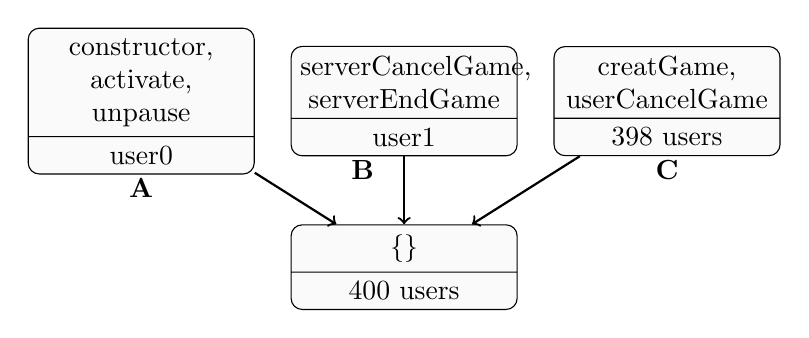
\begin{tikzpicture}%	[edge from parent path=
%	{(\tikzparentnode.north) .. controls +(0,1) and +(0,-1)
%		.. (\tikzchildnode.south)}]
	\tikzstyle{role}=[fill={rgb:black,1;white,50}, draw, rounded corners,
	rectangle split,  
	rectangle split parts=2, 
	rectangle split draw splits=true,  text centered, text width=75]
	\tikzstyle{edge from parent}=[black,<-,thick,draw]
	\node[role] (root) { \{\}  \nodepart{two} 400 users } [level distance = 60, sibling distance=95, grow=up]
	child {node[role] (roleC) {creatGame, userCancelGame \nodepart{two} 398 users }}
	child {node[role] (roleB) {serverCancelGame, serverEndGame  \nodepart{two} user1}}
	child {node[role] (roleA) {constructor, activate, unpause  \nodepart{two} user0}
	};
	\draw ([yshift=-5pt]roleA.south) node[] {\textbf{A}};
	\draw ([yshift=-5pt, xshift=-15pt]roleB.south) node[] {\textbf{B}};
	\draw ([yshift=-5pt]roleC.south) node[] {\textbf{C}};
\end{tikzpicture}
}
\caption{The roles of Dicether.}
\label{fig: DicetherRole}
\end{figure}
Figure~\ref{fig: DicetherRole} shows the mined user roles of Dicether.
Each node represents a role consisting of users at the bottom and associated with different functions.
It is clear that there are three type of separate roles, \textit{A}, \textit{B} and \textit{C}. 
Further, the roles interaction relationship will be investigated in the next section.
%\begin{definition}\label{def: accuracy}
%	\textbf{Role Mining Accuracy.}
%	Given a set of users $U$, and mined user roles $R$, 
%	the heuristic role mining accuracy \textit{Acc} is defined as
%	\begin{align*}
%		&d_1(A, B)  = \sum_{i = 1}^{n} \sum_{j = 1}^{n} | a_{ij} \oplus b_{ij}| \\
%		&Acc =  1 - \frac{\sum_{R_k\in R} \sum_{u_i \in R_k} \frac{1}{n^2}\times d_1( RW[u_i], \sum_{u\in R_k} RW[u])}{||U||}
%	\end{align*}
%Where $A$, $B$ are two $n\times n$ boolean matrices and $\oplus$ is logic xor operator. 
%$DataRW[\cdot]$ is an array of $n \times n$ boolean matrices of data read and data write for all function invocation by $U$. Each cell in a boolean matrix records if a pair of data read and data write exists in function invocation by users. The intuitive behind this accuracy measure is that the users of same role share similar data usage.
%\end{definition}


%In this work, we empirically use 0.9 as the similarity threshold to decide when to merge the roles.  
%According to the function set associated with each user, we group the users to form roles having same function set, which could infer the user cardinality of each role.
%In this work, to explore the security policy of separation of duty, 
%we follow the tradition of role mining to use the inclusion relation of the function sets assigned to roles to define the role hierarchy.
%After mining, the generated roles can construct the basic RBAC model that has no constraints.
%At the time of writing, Dicether has more than 9,427 transactions sent by 400 different users on Ethereum, where a user is an Ethereum external account. 
%Figure~\ref{fig:rolesDicether} shows the mined roles of Dicether.
%For each role, the above is its permission set while the bottom is the set of users  assigned to it.
%There exist five user roles.
%Among them,
%\textit{role1}, \textit{role2}, and 
%\textit{role3} are the user roles with hierarchy,
%where \textit{role2} and \textit{role3} are prior to \textit{role1} and inherit all the permissions from \textit{role1}.
%Hence \text{role2} and \textit{role3} have permissions set:  \{\textit{createGame, userCancelActiveGame}\} and \{\textit{createGame, userEndGameConflict}\} respectively.
%\textit{Role4} has five permissions: \textit{unpause}, \textit{activate}, \textit{activateConflictResolution}, \textit{updateConflictResolution} and \textit{addHouseStake}
%while \textit{role5} have four permissions prefixed with ``server''.
%Reader may contemplate that these roles can be named by ``game player", ``game server'', ``contract owner'', whereas more meaningful but that is not the focus in the paper.
%In this paper, we aim to provide a general approach to reverse engineer the access control model of various smart contracts.
%Although the mined user roles construct as the bedrock of our analysis, the security policies have not been resolved yet.

\subsection{SFSM Learning}
\usetikzlibrary{shapes}
\usetikzlibrary{arrows}
\usetikzlibrary{calc,positioning}
\usetikzlibrary{automata} % LATEX and plain TEX
\begin{figure}[t]
\centering
\scalebox{0.9}{
	\scriptsize
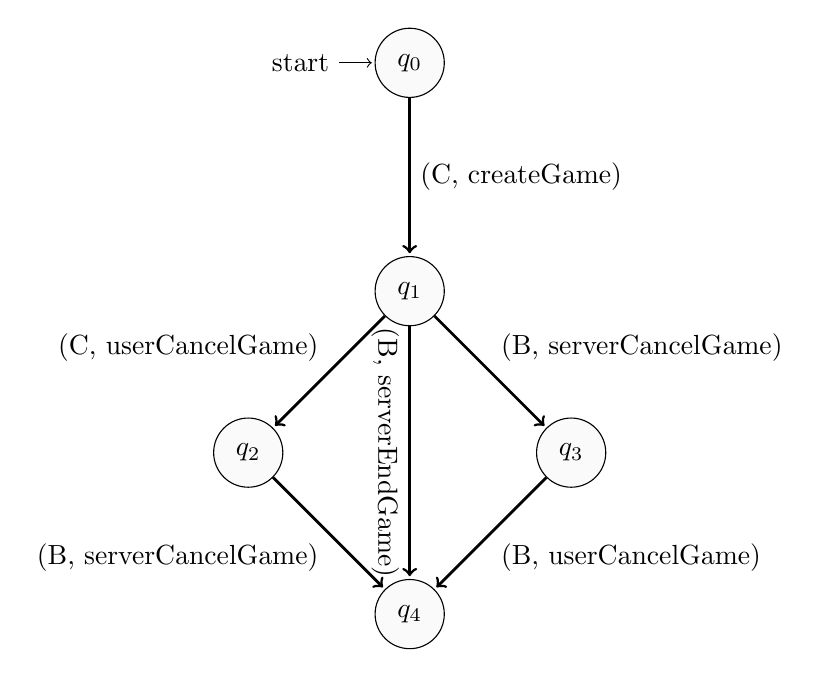
\begin{tikzpicture}[shorten >=1pt,node distance=2.9cm,auto]
	\tikzstyle{every state}=[fill={rgb:black,1;white,50}]
	\node[state,initial] (q0) {$q_0$};
	\node[state] (q1) [below of=q0] {$q_1$};
	\node[state] (q2) [below left of=q1] {$q_2$};
	\node[state] (q3) [below right of=q1] {$q_3$};
	\node[state] (q4) [below left of=q3] {$q_4$};
		
	\path[->, line width=1pt] (q0) edge node {(C, createGame)} (q1)
			  (q1) edge node [swap] {(C, userCancelGame)} (q2)
			  	   edge node {(B, serverCancelGame)} (q3)
	   			   edge node [below, rotate=-90] {(B, serverEndGame)} (q4)
	   		  (q2) edge node [below left] {(B, serverCancelGame)} (q4)   
	   		  (q3) edge node {(B, userCancelGame)} (q4)      
	   			   ;
			  
\end{tikzpicture}
}
\caption{The SFSM of Dicether.}
\label{fig: DicetherSFSM}
\end{figure}
Role-based session finite state machine is inferred via passive learning on the role behaviors within sessions.
To do this, we need to identify sessions and user behaviors within sessions from transaction history.
In smart contracts, session is usually explicitly declared in each function input (e.g., token id for NFT contracts) or implicitly identified by user address.
And we can (semi-)automatically identify sessions with these prior knowledge.
The user behaviors within each session will be further abstracted into role behaviors within each session which can avoid the infinity of user identity.
Each session has only a role behavior sequence which consists of ordered role behaviors in the term of their appearance.
Finally, lots of role behavior sequences are collected from different sessions.
Note that these sequences are all from successful transactions.
Therefore, these sequences construct as positive examples for passive automata learning.
It is difficult to collect negative examples because to prove a function is unreachable for users is infeasible in limited transaction history.

Figure~\ref{fig: DicetherSFSM} shows the role-based session finite state machine of Dicether.
There are five states in total and two roles, \textit{C} and \textit{B} cooperate in gambling games. 
Moreover, the likely temporal property of SFSM can also be identified, such as CTL property: $\textbf{AX}(createGame \implies serverEndGame \lor userCancelGame \lor serverCancelGame)$, though it falls outside of the scope of information security policy studied in this paper.


\subsection{Security Policy Inference}
\label{subsec: informationanlysis}
Roles are associated with functions.
We perform control-flow dependency analysis between functions, which can demonstrate the control-related information flow between roles.
Briefly speaking, for each function, our interests are the state variables used on path conditions and the state variables changed at the end.
%We say information flows from function \textit{A} to \textit{B} if and only if a \textit{A}'s path is dependent on the state variables changed by \textit{B}.
All the control-flow dependency between functions determine the information flow between roles.
We say information flows from role \textit{A'} to \textit{B'} if and only if a path of a \textit{A'}'s function is dependent on the state variables changed by one of a \textit{B'}'s function.
If information can only flow from \textit{A'} to \textit{B'}, information integrity should be satisfied between these two roles.
If no information flows between \textit{A'} and \textit{B'}, separation of duty is satisfied between the two roles.
Further, if information flow within sessions is only allowed over a fixed number of roles, cardinality is implied.

%To determine the security hierarchy of user roles, we perform static analysis of the function set for each role to identify sensitive information and classify user roles into three security levels.
%Recall from Section~\ref{sec:preliminary} that the security hierarchy, for high, medium, and low security, reflects to ability to write sensitive information, read it, or access only non-sensitive information, respectively.
%
%We use information flow analysis for smart contracts to identify sensitive information, which is similar to Ethainter~\cite{...}.
%However, our goal is to find the dominated state variables instead of the sinks in Ethainter.
%Our interested state variables are those used for user permission control (c.f.~\ref{subsec: accesscontrol}).
%Our approach is heuristic; Fig.~\ref{fig: patterns} demonstrates the function patterns we use to identify dominated state variables and also implicitly define the security level of functions.
%The security characteristic of a role is based on the security level of their function set.
%Using this information, the security hierarchy between roles is determined by comparing security characteristics of different roles.
%Specifically, if two roles share a sensitive information set, a role having high security-level functions is prioritized over others having lower security-level functions.
%\begin{figure}[t]
%\begin{tabular}{l@{~}l@{~}l}
%\textbf{high\_func}
%&\textbf{\{}
%$\mathit{stateVar} = \mathit{input}$
%&\textbf{\}}
%\\
%\textbf{medium\_func}
%&\textbf{\{}
%$\mathrm{require}(f(\mathit{stateVar}, \mathit{msg}.\mathit{sender}))$
%&\textbf{\}}
%\\
%\textbf{low\_func}
%&\textbf{\{}
%$\mathit{null}$
%&\textbf{\}}
%\end{tabular}
%\caption{The function patterns (\textit{f} is a boolean function). }
%\label{fig: patterns}
%\end{figure}
%
\usetikzlibrary{shapes}
\usetikzlibrary{arrows}
\usetikzlibrary{calc,positioning}
\begin{figure}
\centering
\scalebox{1}{
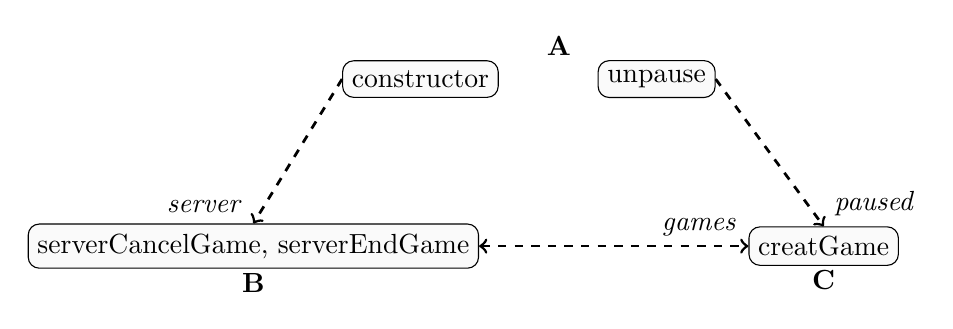
\begin{tikzpicture}[node distance=3cm]
	\tikzstyle{role}=[fill={rgb:black,1;white,50}, draw, rounded corners,
	rectangle split,  
	rectangle split parts=1, 
	rectangle split draw splits=true,  text centered, text width=]
	\node[role] (roleA1) {constructor};
	\node[role] [right of=roleA1] (roleA2) {unpause};
	\node[role] [below right of=roleA2] (roleC) {creatGame};
	\node[role] [below left of=roleA1] (roleB) {serverCancelGame, serverEndGame};

	\draw ([xshift=50pt, yshift=5pt]roleA1.north) node[] {\textbf{A}};
	\draw ([yshift=-5pt]roleB.south) node[] {\textbf{B}};
	\draw ([yshift=-5pt]roleC.south) node[] {\textbf{C}};
	
	\draw [->, dashed, line width=1pt] (roleA1.west) -- (roleB.north) node[above left] {\textit{server}}; 
	\draw [->, dashed, line width=1pt] (roleA2.east) -- (roleC.north)
	node[above right] {\textit{paused}}; 
	; 
	\draw[<->, dashed, line width=1pt] (roleB.east) -- (roleC.west) node[above left] {\textit{games}}; 
	
\end{tikzpicture}
}
\caption{The information flow between roles of Dicether.}
\label{fig: DicetherRoleInformationFlow}
\end{figure}
Figure~\ref{fig: DicetherRoleInformationFlow} shows information flow between the three aforementioned roles of Dicether.
Role \textit{B} depends on the \textit{server} specified by role \textit{A} in constructor function,
while role \textit{C} depends on the value of \textit{paused} as well.
And only role \textit{B} and \textit{C} communicate within game sessions.
Hence, there exists several likely security policy,
i.e., (1) Integrity, $
\square (role(msgsender)!=A)\implies \square (server_0=server)
$ and
$
\square (role(msgsender)!=A)\implies \square (paused_0=paused)
$
and (2) Cardinality, $
\square (role(msgsender)!=B\land role(msgsender)!=C)\implies \square (games_0=games)
$.
%\subsection{Security Policies Inference}
%\label{subsec:inferconstraints}
%
%
%\begin{figure*}[t]
%	\centering
%	%	\hspace{-56pt}
%	\includegraphics[scale=0.43]{Figures/Chapter4/Dicether-sessionTraceSummaryWithUser.pdf}
%	\caption{The session model learned from Dicether history.}
%	\label{fig:dicether-SessionModel}
%\end{figure*}	
%
%
%
%\begin{algorithm}[t]
%\caption{Infer constraints of RBAC model }
%
%\begin{algorithmic}[1]	
%		\Require $S$: a transaction sequences set representing sessions
%		\Require $U$: a users set; $R$: a roles set 
%		\Require $Threshold \ge 1$: the maximum of valid cardinality
%		
%		\Procedure{InferConstraints}{$S, U, R, Threshold$}      
%		\State $C \gets \emptyset$ \Comment{a set of constraints} 
%		\State $Card_u, Card_r, Card_h \gets 0, 0, \emptyset$ \quad
%		\State $SSD, DSD \gets True, True$ \quad
%		
%		\State $A \gets \textsc{LearnAutomata}(S)$
%		\State $W \gets \textsc{InferWorkflow}(S, A, R)$
%		
%		\ForAll{user in $U$}
%		\If{$\exists r1, r2 \in R \, (r1 \ge r2)\land$ \textit{a user has r1, r2}}
%		\State	$SSD \gets False$
%		\EndIf
%		\EndFor
%		
%		
%		\ForAll{path in $W$}
%		\State $Card_u \gets \max(Card_u, numOfUsers(path))$ 
%		\State $Card_r \gets \max(Card_r, numOfRoles(path))$  
%		\ForAll{$r$ in $R$}
%		\State $Card_h(r) \gets \max(Card_h(r),$ 
%		\State $\qquad \qquad \qquad numOfUsersWithRole(r,path))$ 
%		\EndFor
%		\If{$\exists r1, r2 \in R \, (r1 \ge r2)\land$ \textit{(a user has r1, r2 at path)}}
%		\State $DSD \gets False$
%		\EndIf
%		\EndFor
%		
%		\If{$Card_u \le Threshold$}
%		\State $C \gets C \cup \{Card_u\}$
%		\EndIf
%		\If{$Card_r \le Threshold$}
%		\State $C \gets C \cup \{Card_r\}$
%		\EndIf
%		
%		\ForAll{$Card_h(r) \in Card_h$}
%		\If{$Card_h(r) \le Threshold$}
%		\State $C \gets C \cup \{Card_h(r)\}$
%		\EndIf
%		\EndFor
%		
%		\If{$SSD = True$}
%		\State $C \gets C \cup \{SSD\}$
%		\EndIf
%		
%		\If{$DSD = True$}
%		\State $C \gets C \cup \{DSD\}$
%		\EndIf
%		
%		\State \Return $C$ 
%		\EndProcedure
%		
%		\Procedure{LearnAutomata}{S}
%		\State Extract function sequences from transaction sequences
%		\State Use passive automata learning alogrithm 
%		\State \Return $A$ \Comment{a finite state machine}
%		\EndProcedure
%		\Procedure{InferWorkflow}{S, A, R}
%		
%		\State Rename users in each transactions sequence of $S$ in the order of their appearance and keep theirs roles in $R$
%		\ForAll{path in $A$}
%		\ForAll{transition $t$ in path}
%		\State $t \gets t\cup {usersAndRolesOfTxSeqsMatch(path)}$
%		\EndFor
%		\EndFor
%		\State $W \gets A$
%		\State \Return $W$ \Comment{session workflow automata}
%		\EndProcedure
%		
%	\end{algorithmic}
%	\label{algo:inferConstraints}
%\end{algorithm}
%In this section, we will illustrate how to infer the separation of duty and cardinality constraints
%from the collected user access logs.
%In recent years, there are many approaches for constrained role mining which minimize the number of roles as well as explore the constraints include cardinality constraint. 
%Inspired by these,
%Algorithm~\ref{algo:inferConstraints} introduces a novel approach to infer the constraints including separation of duty and cardinality.
%To extract the transaction sequences within sessions for one of the algorithm inputs,
%we need to identify sessions first.
%Our experience is that smart contracts of cycle or parallel transition types mentioned in Sect.~\ref{subsec: transaction} usually have multiple homogeneous processes which finish similar tasks such as the games of Dicether in Sect.\ref{sec:motivationExample}.
%Generally, each task has a unique identity.
%We rely on these explicit task identities to split access logs into different sessions where each session consists of an ordered transaction sequence in the order of appearance.
%
%Given a transaction sequence set $S$, a users set $U$ and a roles set $R$, as well the customized maximum cardinality $Threshold$, the algorithm first initializes a constraints set $C$ and $Card_u$, $Card_r$ and $Card_h$ for users, roles and hybrid cardinality respectively (Line 2-3).
%The constraints: the static separation of duty ($SSD$) and the dynamic separation of duty ($DSD$) are assumed true at the first (Line 4).
%The algorithm then first learns a finite state machine model with respect to function sequence information using passive automata learning (Line 5).
%Later the model is extended to form a session workflow model by adding users and roles information (Line 6) like fig.~\ref{fig:dicether-SessionModel}. 
%According to the aforementioned formulas and calculations defined in Sect.~\ref{subsec: constraints}, we validate $SSD$ and $DSD$ and also retrieve $Card_u$, $Card_r$ and $Card_h$ (Line 7-17).
%Further, the retrieved $Card_u$, $Card_r$ and $Card_h$ are validated by the customized $Threshold$ and all validated constraints are added to the constraint set $C$ (Line 18-29), as the result of this algorithm.  
%
%To gain the access control constraints of Dicether, 
%we need to learn a session model from access logs existing in the transactions history.
%There are a lot of game sessions of which each is identified by explicit \textit{gameId}.
%Figure~\ref{fig:dicether-SessionModel} shows the inferred session model of Dicether.
%Figure~\ref{fig:dicether-SessionModel} demonstrates that the session model has 12 states and 14 transitions.
%For each state node in the model, the right above is the function set while the right bottom shows the user set and the corresponding role sits on the left side. 
%In this model, each path corresponds to a session similarity pattern discovered in the history.
%For example, a session $\{(user2, creategame)$, $(user3, serverEndGame)\}$ for game $ID_i$ is similar to another session of $\{(user4, createGame)$, $(user3, serverEndGame)\}$ for game $ID_j$, where the two sessions will be represented by abstracted pattern  $\{(u1, role1, creategame)$, $(u2, role5, serverEndGame)\}$.
%
%For each session, Figure~\ref{fig:dicether-SessionModel} indicates there are two different users labeled by $u_1$ and $u_2$. 
%As for the user roles for each session, we notice that the active roles are either $\{role1, role5\}$,
%or $\{role1, role2, role5\}$ or $\{role1, role3, role5\}$.
%When we consider the factors that it is the same user, namely $u1$ who has $role1$ and $role2$ as well $role1$ and $role3$, and $role2$ and $role3$ are prior to $role1$.
%We can summarize that for each session the number of active roles are two and these active roles are either  $\{role1, role5\}$,
%or $\{role2, role5\}$ or $\{role3, role5\}$.
%
%Recall that the constraints are not limited to facilitate the contract migration into RBAC systems. 
%The constraints are useful for the vulnerability detection of smart contracts. 

\subsection{Testing}
\label{subsec: testing}
%\paragraph{What to test?}
The goal of testing is to detect vulnerabilities on the aforementioned security policies.
\paragraph{Test Oracle}
Given a integrity property $\varphi$: $
\square (I_{h}^{0} = I_{h})\implies \square (O_{h}^{0} = O_{h})
$,
the testing attempts to generte an counterexample which satisfies $!\varphi$: $ 
\square (I_{h}^{0} = I_{h}) \land \Diamond (O_{h}^{0} != O_{h})
$.
However, it is difficult to automatically test this temporal property
because testing usually relies on atomic propositions as the test oracles, such as reentrancy~\cite{atzei2016survey}, delegate call~\cite{jiang2018contractfuzzer} and etc..  
To do that, we need to reduce $\varphi$ into practical test oracle $t$.
The $\square(I_{h}^{0} = I_{h})$ can be eliminated by $role(msgsender)!=h$ without loss of precision, where \textit{msgsender} is the caller to contract functions.
Then, $\Diamond (O_{h}^{0} != O_{h})$ could be over-approximated by function reachability propositions $\overset{f_o}{\lor} {f_o}$,
where $f_o$ refers to the function that could change $O_h$.
For separation of duty and cardinality, the approach is similar.
\begin{figure}
	\centering
	\begin{tabular}{l@{~}l}
		\textbf{while}( true )\{ & \\
		\; \; contract = \textbf{replay}( history ); & \\
		\; \; \textbf{for}( i: 0..k )\{ & \\
		\; \; \; \; user, function = \textbf{tcgeneration}( ); & \\
		\; \; \; \; reach = \textbf{symexec}( contract, user, function ); & \\
		\; \; \; \; \textbf{checkAndReport}( reach );&\\
		\}\}&\\  
	\end{tabular}
	\caption{Smart contract testing}
	\label{fig: testing}
\end{figure}
\paragraph{Test Environment}
As for shown in fig.~\ref{fig: testing}, 
first \spcon will replay all transaction history of smart contract to keep contract state close to its running environment on Ethereum.

\paragraph{Test Case Generation Strategy}
Because it is infeasible to generate every possible transaction sequences,
we limit the capability of \spcon to generate transaction sequence of length up to \textit{k}.
Further, the functions in a transaction sequence can also be partially ordered according to their control-flow dependency relationship, which can reduce unnecessary test cases.
Then, \spcon uses symbolic execution to under-approximate the function reachability problem.
Finally, \spcon checks and reports an counterexample if there is violation against the aforementioned test oracles.
%
%We test smart contracts for vulnerabilities based on the breaches of security policies of user permission inferred from the history and the information flow of the smart contract.
%We exploit potential user accesses that were not observed in the history and then generate and execute a test harness programs for validating security policies of the smart contract.
%\begin{definition}
%\textbf{User Permission Attack Detection.}
%Given smart contract history $H$ and a likely user permission policy $\varphi$, find a future attack witness $\pi^{+}:  < (r_1, f_1), (r_2, f_2), \ldots, (r_n,  f_n)>,\; r_i\in R,\; f_i \in \mathit{ABI}$ such that 
%%\todo[inline]{CA: consider using $f$ over $fun$.}
%\begin{align*}
% \exists \pi^{+} (H \implies \varphi) \land (H \triangleright \pi^{+}  \implies \neg\; \varphi) 
%\end{align*}
%%If we can find an attack vector, we will manually verify the result and confirm if it reveals a true security vulnerability.
%\end{definition}
%
%Take integrity as an example, suppose that a baseline execution trace of \textit{H} is $\pi:  < (r_h, f_1), (r_h, f_2), \ldots, (r_h,  f_n)>$ where $r_h$ refers to the high security-level role 
%as well as a possible $\pi^{'} = \pi \triangleright \pi^{+}$.
%According to integrity policy expressed via HyperLTL property in Sect.~\ref{sec:preliminary} , if the final state changes by $r_h$ on execution traces $\pi$ differentiate from the corresponding state changes on execution traces $\pi^{'}$, 
%the integrity policy is violated and then $\pi^{'}$ is an attack witness.
%
%Finding an attack witness $\pi^{'}$ is nontrivial since contract in its nature, is a never-stop state transition system and it is impossible to enumerate every possible execution trace.
%To overcome this challenge, we reduce functions under consideration to those related to information flow between roles of the permission policy under test and order functions in an execution trace according to their control-flow dependency relation or a state machine model (session).
%With these improvement, we can largely minimize the size of possible execution traces.
%Nonetheless, there remains a combinational explosion problem for $\pi^{'}$ selection.
%To mitigate this problem, we seek a \textit{k}-bounded solution where \textit{k} new function calls will be inserted into $\pi^{+}$.
%
%\liu{Algorithm for test case generation}
%
%Given a smart contract, 
%\spcon will iterate all the transaction sequence of length up to $k$ for finding violations of \textit{Policy}.
%%It is possible that a bug of contract can be triggered only by the attack vector beyond $k$-transactions sequence.
%In most cases, attackers trigger attacks using a small number of transactions, i.e., $k$ is very small.
%%And for simplicity, we consider 
%\begin{figure}[t]
%	\centering
%	\includegraphics[scale=0.9]{Figures/Chapter4/TestHarness.pdf}
%	\caption{The test harness in \spcon.}
%	\label{fig: harness}
%\end{figure}
%
%\spcon uses symbolic execution to test smart contracts.
%As shown in Fig.~\ref{fig: harness}, firstly, \spcon automatically replays all the concrete transactions of a smart contract history so that the tested smart contract instance is a snapshot of that on Ethereum.
%Secondly, \spcon executes the test harnesses of $k$-transaction calls with symbolic users and symbolic functions as input to validate concrete security policies of the smart contract.
%Finally, \spcon can iterate all the possible $k$-transaction calls to find the candidates of attack vectors.
%
%To avoid the combinatorial explosion up to $(||U|| \times ||\mathit{ABI}||)^k$ test cases, we minimize $||U||$ by selecting small number of users as representatives for different mined user roles in Sect.~\ref{subsec: rolemining}.
%Further, we use the data-flow and control-flow analysis of smart contract functions to prevent unnecessary function combinations, thus reducing our test effort without the loss of generality and accuracy. 
%
%After symbolic execution, the attack candidates are sorted in a predefined ranking method.
%The rank of an attack candidate is determined by the attacker role and the attacked role.
%Figure~\ref{fig: risk} shows the risk rank for attack candidates of smart contracts.
%%The first column is the role of the attacker, either permissionless role or permissioned role ,
%%while the second column is the attacked role.
%The permissioned roles check user permission when user calls one of the functions associated with the roles, 
%while the permissionless does not check it.
%If the attacker is from permissionless role and the attacked role is permissioned role,
%the risk of the attack candidate is very high.
%And if a permissioned attacker attacks a permissoned role, the risk is very low. 
%The security policy is of high risk if the attacker could be any roles, 
%while of medium risk if the attacker is from limited roles.
%If \spcon cannot find any attack, we believe that the risk of security policy is very low.
%We manually confirm if these attack candidates can trigger real world attack.

%\begin{figure}
%\centering
%\includegraphics[scale=0.7]{Figures/Chapter4/RiskofAttack.pdf}
%\caption{The risk rank of attack candidates of user permission.}
%\label{fig: risk}
%\end{figure}


\subsection{Abstraction and Model Checking}
%\liu{Abstraction. Abstract Contract Model}
\usetikzlibrary{shapes}
\usetikzlibrary{arrows}
\usetikzlibrary{calc,positioning}
\usetikzlibrary{automata} % LATEX and plain TEX
\begin{figure}[t]
\centering

\begin{subfigure}[b]{0.50\columnwidth}	
%	\scalebox{0.5}{
	\scriptsize
	\begin{tikzpicture}[shorten >=1pt,node distance=1.55cm,auto]
		\node (userCancelGame) {	
			\begin{lstlisting}[language=Solidity, basicstyle=\tiny]
		function userCancelGame() public payable
		{
			require(games[msg.sender]!=ENDED);
			if (games[msg.sender]==ACTIVE){
				games[msg.sender] = USECANCEL;
			}else if (games[msg.sender]==SERVERCANCEL){
				games[msg.sender] = ENDED;
			}else{
				revert();
			}
		}
			\end{lstlisting}
		};
	
	\end{tikzpicture}
%	}
\end{subfigure}
\hfill
\begin{subfigure}[b]{0.48\columnwidth}
\scalebox{0.8}{
	\scriptsize
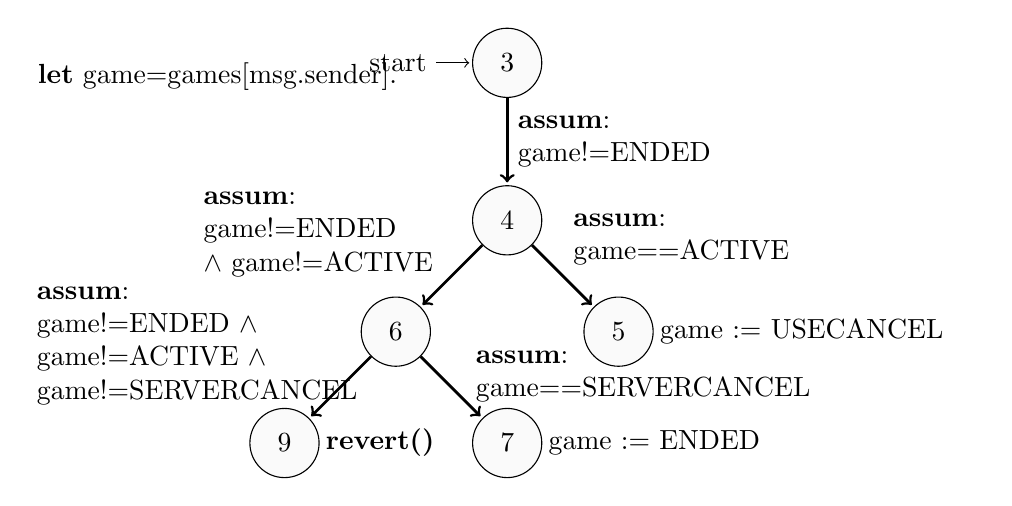
\begin{tikzpicture}[shorten >=1pt,node distance=2cm,auto]
	\tikzstyle{every state}=[fill={rgb:black,1;white,50}]
	\node[state,initial] (q0) {$3$};
	\node[state] (q1) [below of=q0] {$4$};
	\node[state] (q2) [below right of=q1] {$5$};
	\node[state] (q3) [below left of=q1] {$6$};
	\node[state] (q4) [below right of=q3] {$7$};
	\node[state] (q5) [below left of=q3] {$9$};
	
	\node[text width=4cm, xshift=15pt] (line5) [right of=q2] {game := USECANCEL};
	\node[text width=4cm, xshift=15pt] (line7) [right of=q4] {game := ENDED};
	\node[text width=4cm, xshift=15pt] (line7) [right of=q5] {\textbf{revert()}};
		
	\path[->, line width=1pt] (q0) edge node[text width=2cm] {\textbf{assum}: game!=ENDED} (q1) 
							  (q1) edge node[text width=2cm] {\textbf{assum}: game==ACTIVE} (q2) 
							  (q1) edge node[text width=3cm, yshift=15pt, xshift=10pt, left of=q1] {\textbf{assum}: game!=ENDED $\land$ game!=ACTIVE} (q3) 
  							  (q3) edge node[text width=3cm, xshift=5pt, yshift=-9pt] {\textbf{assum}: game==SERVERCANCEL} (q4) 
  							  (q3) edge node[text width=3cm, yshift=15pt, xshift=-10pt, left of=q1] {\textbf{assum}: game!=ENDED $\land$ game!=ACTIVE $\land$ game!=SERVERCANCEL} (q5) 
	 ;
 	\node (label) [yshift=-5pt, xshift=-70pt, above of=q1, text width=7cm] { \textbf{let} game=games[msg.sender]. };			  
\end{tikzpicture}
}
\end{subfigure}


\caption{The control flow graph of Dicether's \textit{userCancelGame}.}
\label{fig: abstractionDicetherFunction}
\end{figure}

\begin{definition}
	\label{def: contractmodel}
	\textbf{Contract Model.} 
	A contract model $\mathit{M}$ can be defined by $(\delta_0, F, \Delta, T)$ where $\delta_0 \in \Delta$ is initial state of contract, $f \in  F$ is a public function of contract and $T \subseteq \Delta \times F \times \Delta $ is transition function of contract state.
\end{definition}
The initial state of contract is actually the abstraction of contract state at current transaction history.
As stated before, only successful function invocation can change contract state.
%	Further, the reachability of function is decided by predicates over current contract state instead of its input. 
Each path of function can be abstracted by a boolean program: $Path(f)\implies Precondition() \land StateChanges(\Delta_1)$,  where \textit{Precondition()} is a set of satisfied predicates and \textit{StateChanges($\Delta_1$)} is a set of assignments of state variables.
Figure~\ref{fig: abstractionDicetherFunction} shows the control flow graph of Dicether's \textit{userCancelGame} function.
The program path ``Line 3 $\rightarrow$ Line 4 $\rightarrow$ Line 5'' can be abstracted by ``\textit{\textbf{assume}: game==Active; game:=USERCANCEL}''.
That means when the game is at active status, user can call \textit{userCancelGame} to transit the game to user cancellation status.

It is impractical to get a precise abstraction of all contract semantic.
For example, the inter-contract call inside functions is hard to abstract because there exists state explosion problem for a cross-contract model even all the inter-contract calls are statically determined.
Therefore, in this paper, we derive a safe abstraction following interpolant lemma~\cite{craig1957three} to get an over-approximated abstract model for smart contracts.
We say it is a safe abstraction if the property is true on the original model then it is true on the abstract model.
We argue the over-approximated abstract model is also sound since the information security property relates to the state changes of smart contracts, which is precisely modeled instead. 

Finally, the abstract model and security properties are verified by the state-of-art symbolic model checking tool, e.g., NuSMV~\cite{cimatti1999nusmv}. 
If property holds, we say this property is proved and can further be added to the specification of smart contracts.
Otherwise, we can symbolically execute or manually check the generated counterexample by model checking to confirm whether it is a true counterexample.
%
%We divide predicates used for global variables checking into the following four categories:
%\begin{itemize}
%	\item \textbf{compared with trivial transaction input.} These trivial transaction input includes the transferred ether and function input. For example, $require(balance[msg.sender] >= amt)$ is used for ERC-20 token transfer function which specifies amount to transfer his/her token to others.
%	This predicate indicates that any user cannot transfer token of \textit{amt} larger than his/her account balance. 
%	However, this case won't affect the reachability of function since user can adjust the given \textit{amt} to pass the check and we aggressively have  $f\implies StateChanges(\Delta_2)$.
%	
%	\item \textbf{compared with transaction sender.}
%	The transaction sender includes \textit{tx.origin}, the creator of initial transaction, and \textit{msg.sender} of every message call to contracts.
%	A user cannot modify the value of \textit{tx.origin} and \textit{msg.sender}.
%	Therefore, this case like $require(msg.sender == owner)$, will influence whether a user can reach a function successfully and we have $f\implies Precondition(\Delta_1) \land StateChanges(\Delta_2)$.
%	\item \textbf{compared with constant variable.}
%	State machine-based smart contract design is recommended to prevent illegal function access.
%	For example, $\{Escrow.state == X | X \in \{OPEN, SUCCESS, REFUND\}\}$ is used in \textit{CrowdSale} contract from OpenZeppelin library, where user access is only allowed for limited functions at a specific state.
%	Because this type of predicates is irrelevant to user, it will control user access to contract functions  and we have $f\implies StateChanges(\Delta_2)$.
%	
%	\item \textbf{compared with environment variable.}
%	The blockchain environment variables such as \textit{block.number}, \textit{block.timestamp} are usually used as soft clock or random seed of contracts. 
%	However, these variables can be manipulated by miner.
%	This will introduce great uncertainty if contract' access control relies on environment variables.
%	For simplicity, we do not take the predicates related to environment variables into consideration in this paper and we aggressively have $f\implies Precondition(\Delta_1) \land StateChanges(\Delta_2)$.
%\end{itemize}
%
%Above, we consider \textit{Precondition($\Delta_1$)} for the predicates, i.e., the comparison between global variables and transaction sender as well as constant variables, which is usually to restrict user access.



